\documentclass[11pt,preprint]{aastex}
\usepackage{amsmath}
\usepackage[top=1in, bottom=1in, left=1in, right=1in]{geometry}
%\usepackage{natbib}
%\usepackage{natbibspacing}
\usepackage{enumitem}
\usepackage{url}
\usepackage{xcolor}
\setlist[itemize]{noitemsep, topsep=0pt}
\setlist[enumerate]{noitemsep, topsep=0pt}
%\setlength{\bibspacing}{0pt}
\setlength{\parskip}{0pt}
\setlength{\parsep}{0pt}
\setlength{\headsep}{6pt}
\setlength{\topskip}{0pt}
\setlength{\topmargin}{0pt}
\setlength{\topsep}{6pt}
\setlength{\partopsep}{0pt}
\setlength{\footnotesep}{8pt}

\begin{document}
\def\simlt{\lower.5ex\hbox{$\; \buildrel < \over \sim \;$}}
\def\simgt{\lower.5ex\hbox{$\; \buildrel > \over \sim \;$}}
\def\wLO{\omega_0}

\title {LAB 1: Exploring Digital Sampling, Fourier Filtering, and Heterodyne Mixers}

\tableofcontents


\section{Introduction}

\noindent
In this lab, we experimentally investigate digital
samplers, discrete Fourier Transforms, and mixers. These are 
tools of the trade in radio astronomy, and
you use them every day when you use a cell phone, listen to the radio,
or watch television. Did you know that WiFi was invented by a radio
astronomer?

To get firm footing in the methods of radio astronomy, you will perform a series of
experiments that illustrate the utility and hazards of these various techniques. 
You will configure equipment in the lab, acquire and analyze data, and store and illustrate the results.
The signal processing pipeline you build in this lab will be re-used in Lab 2 to
observe 21-cm line emission from hydrogen in the Milky Way, so 
put in the time to make it work and understand it. The effort you
invest now will pay dividends later in the class.

This first lab is an excellent time to establish good research and laboratory practices.
Remember that your grade is determined by the report you turn in
three weeks from now. All of the exercises that follow are aimed at building your
understanding and giving you the raw materials (and data) from which to build that report.
You don't have to finish everything, or proceed in the in order presented, but you do have
to write a quality report that addresses the goals in \S\ref{goals}.

Here are some specific suggestions for turning these lab instructions into a successful report:
\begin{itemize}

\item Keep careful notes, preferably in a {\bf lab notebook} that you write in as you hook things up.
Good notes document how the data are derived from the experimental setup so you can describe it accurately and track down mistakes.
If you show your knowledgable GSI a head-scratcher of a plot but cannot remember
which port of the mixer you plugged the noise into, they may have trouble diagnosing your problem.

\item Back up (or revision control) your data, code, and plots. Nothing is more demoralizing than having to redo work
or being unable to reproduce a result you need.

\item Start your report early. If you plan for which equipment, data, and plots you need
for your report, you will spend your time more efficiently and avoid the 
panic of writing up at the last minute.

\item Formal lectures, the pages linked on AstroBaki, and these lab instructions are 
resources to help you write a strong report. As in real-life research, there
is no one textbook containing everything you need to know. Explore, take notes, and show
me what you learned in your report. Remember, I can only grade you on what you write down.
Make sure what you write down is your own work, in your own words. Cite sources
external to this class (no need to cite AstroBaki, lecture, or the lab instructions).

\item Your reports will be in the style of scientific publications. They are narratives of explanation and discovery 
that bring the reader---a science colleague---to the point of understanding and having confidence in your results.
You are presenting your work, but this report is about the {\it reader's} journey, not yours.
It is a presentation of synthesized results with the background and salient details necessary to understand them. 
It is {\it not} a play-by-play of everything you did, all the plots you made, and all of the wrong turns along the way.

\end{itemize}


\section{Goals} \label{goals}

\noindent
The goals of this lab---the results your report should
demonstrate you have achieved---are as follows.

\begin{itemize}

\item Sample electronic signals and convert them into digital signals. Demonstrate
the phenomenon of aliasing and quantitatively relate that to the Nyquist criterion.

\item Correctly use and display Discrete Fourier Transforms (DFTs) to 
  determine the frequency power spectrum of a time
  series. Correctly calculate and label frequency and power axes in plots and demonstrate
  understanding of how frequency ranges and resolutions are determined from the duration and 
  cadence of samples in a time series.

\item Demonstrate understanding of negative frequencies. Motivate and measure how complex inputs to a Fourier Transform
break the positive/negative frequency degeneracy.

%\item Learn about the Fast Fourier Transform (FFT) as a fast
%  implementation of the DFT.

\item Identify and characterize noise in electronic measurements and explore how it behaves 
  under the Fourier Transform.

\item Apply the convolution/correlation theorem, explain how
  spectral leakage in a power spectrum can be understood in this framework,
  and test the relationship between autocorrelation functions and power spectra.

\item Derive the basics of mixing for frequency conversion
  (the heterodyne technique) and explore how electronic mixers differ from
  ideal ones. Construct double- and single-sideband mixers and use measurements
  to demonstrate the theoretical and practical differences in their operation.

\end{itemize}

\noindent
In order to achieve these goals, you must develop many new technical skills.
These need not be written about explicitly in your report; the quality of
the report will itself demonstrate your growing proficiency. These technical skills include:

\begin{itemize}

\item Using the Python programming language for analysis, signal processing, and plotting,

\item Learning enough \LaTeX to write up your results in a formal lab
  report that including an abstract, captioned figures, tables, and citations.

\item Gaining familiarity with configuring laboratory equipment 
and navigating the computing environment.

\end{itemize}

\section{Schedule}

\noindent
This is an ambitious lab with a steep learning curve.
It is important not to get behind or backload your work schedule.
In particular, writing the report takes a lot longer than you might think.
\begin{enumerate}

\item {\it Week 1.} Finish \S
  \ref{nyquist} and read the accompanying
  material in \S \ref{pwrspectrum}. {\it Be prepared to show work, 
  software, and results to the class.}

\item {\it Week 2.} Finish \S
  \ref{mixersect} and read \S \ref{hetereo}. Again, be prepared
  to present to the class.

\item {\it Week 3.} Read the handouts in \S
  \ref{report} and write your formal report.  Refer to
  our handouts and linked material for tips on how to structure
  a scientific paper. You will be graded on the degree to which your
  report addresses the specific goals in \S\ref{goals} and conforms to
  standards of a quality scientific publication.

\end{enumerate}

\section{Software Engineering}

\noindent
The programming required to complete these labs will increase in scale throughout the semester.
As it does, you will need to learn to organize, document, test, and stabilize your code.  The process
of building sound code is broadly referred to as software engineering, and
it may be one of the most marketable skills you learn in this class.

Learning to engineer good software can take a lifetime, but let us start with a few
principles in this lab.

\begin{itemize}

\item {\it Package your code}.  Keep files containing code together in 
directories that are separate from the data you acquire.  
Organize your code into functions and classes, and put the definitions in separate, importable files called modules.  
Modules separate the definition
of the code from the scripts and notebooks you use to execute code with changeable parameters. Packaging code vastly improves
organization, testability, and the degree to which you can re-use good code. Functions, classes, modules, and installable {\bf packages}
are easy to implement in Python, and there are many resources online to teach you how to use them. 

\item {\it Code (at least) twice}. It is nearly impossible to write well-organized code while figuring
something out for the first time. You need room to hack at the problem, try and fail, learn and iterate.
Code once to get a sense of how your program should work, then
re-code it to get the organization and interfaces right. Time spent organizing and testing code up front will pay
dividends later.

\item {\it Test your code.} How do you know your code is doing what it should? Yes, it may run
without raising an exception, but that doesn't mean it did what you intended. In software as in science,
you can only trust something to the extent that you have tested it.
Keep your tests organized so that you know what you have tested, and how. Modular testing (a.k.a 
{\bf unit testing}) is the key to success in large
software projects, particularly ones involving multiple people. The {\tt unittest} module is 
commonly used in Python, but other modules have their own merits.

\item{\it Control your revisions}.  {\bf Revision control} uses a specialized program ({\tt git} is popular) to
track the changes made to your code. They allow you to edit code with impunity, knowing that you can
always ask for a report on what you changed and where, and you can always backtrack to a previously committed
state of the code if you screw something up.
I suggest opening a (free) GitHub account, initializing a project
for this class, and then committing to it regularly.  GitHub works with {\tt git} to back up your work remotely, and it also 
allows you to easily synchronize your work across multiple computers.  It is seriously worth the learning curve.

\end{itemize}

\noindent
Advanced software engineering combines all of the steps outlined above, using online repositories to hold various
branches of a software project, and when any of a community of coders push their changes, a continuous integration system runs
unit tests on the code to make sure that nothing was broken, that the new codes defines new tests it must pass, and that
all the code conforms to reasonable documentation and legibility standards.  Code reviews examine changes that are
made and submitted through pull requests, and then the changes (often multiple in parallel) are merged into the master code base of the
project.

We don't need the advanced machinery for this class, but it is good to be aware of how coding communities work and
to start down the path of good coding practices yourself. Try to improve your software engineering practices using the
suggestions above.

{\it At a minimum, firmly separate data acquisition (the code that runs and interacts with
equipment in the lab and at the telescope) from data analysis}.  For the former, scripts that run from the command line
are most appropriate. For the latter, {\tt jupyter} notebooks are a fantastic tool. If you have code that needs to
run under both environments, write modules that you can import into either.


\section{Digitally Sampling a Sine Wave (Lab Activity, Week 1)}
\label{nyquist}

\subsection{Handouts and Software}

\noindent
Your work this first week will require you to navigate
the Linux operating system, using your (Vi/Emacs/3rd party) text editor to write Python. 
On Astrobaki\footnote{\url{https://casper.ssl.berkeley.edu/astrobaki/index.php/Undergraduate\_Radio\_Lab}}
we have linked primers on
Linux/Unix, Python Installation and Basic Programming, Unix Text Editors, and Revision Control.  You can
also review the key course content for this week: Nyquist Sampling and the Fourier Transform.

%\subsubsection{Handouts}
%\begin{enumerate}
%\item Learning Linux: {\tt unixprimer.pdf} ``A SHORT UNIX PRIMER'' Basic
%  commands for Linux/Unix operating systems. Eventually you'll want to
%  know all of the commands in here because they are so useful.
%
%\item Learning the EMACS editor: {\tt emacs-beg.pdf} {\it ``A Beginners
%  Guide to Emacs''} and the related {\tt emacskeyops.pdf} ``Common
%  Editing Tasks and Their EMACS Keystroke Counterparts''. Emacs is
%  excellent for everything, including editing writing computer
%  code. Efficient editing means using the keyboard instead of the mouse;
%  the second handout gives keystroke commands for the most commonly
%  needed editing sequences.
%
%\item Getting into Python: {\tt idltut1\_ay121.pdf} {\it ``Quick Python
%  Tutorial Number One for AY121''} Gives you the basics of Python.
%
%\item Plotting in Python: {\tt bpidl.pdf} {\it ``BPPython---BASIC PLOTTING IN
%  Python: PLOTS, MULTIPLE PLOTS, COLORS, MAKING POSTSCRIPT FILES''} Sections
%  1 and 2 are enough for now.
%
%\item {\it This handout is optional}, because for this lab you can get
%  along with just the material below in \S \ref{pwrspectrum}. This handout
%  is more detailed, 28 pages of all you need to know about Discrete
%  Fourier transforms.  {\tt fourierc.pdf} {\it ``DISCREETLY FINE TIMES
%    with DISCRETE FOURIER TRANSFORMS (DFT’s with DFT’s) or “WHY DOES
%    THAT FFT OUTPUT LOOK SO sWEIRD???” ''}.
%\end{enumerate}
%
\subsubsection{The {\tt ugradio} Python Package}

\noindent
{\bf Modules} are a way to distribute and reuse Python code.  They are themselves
just bundles code that you {\tt import} into your program, where you can
access everything as if you'd written it yourself.  {\bf Packages} are bundles
of modules that can all be installed together.  For this class, we will be using
the {\tt ugradio} package to provide supporting code for your labs.  This package
is already installed on the lab computers (you can test this by opening {\tt ipython}
and typing {\tt import ugradio}).  If you ever need to install it on another computer,
all of the code is on GitHub and linked to from the course website.  

You will make use of two modules inside of the {\tt ugradio} package: {\tt pico}, and {\tt dft}.
Take a minute to browse the code in these two modules so that you understand how to use it.

\begin{itemize}

\item {\tt ugradio.pico} --- runs the PicoSampler Analog-to-Digital Converter to digitally sample signals. This is essential.

\item {\tt ugradio.dft} --- provides code for doing arbitrary Discrete Fourier Transforms.  This
contrasts the functionality of {\tt numpy.fft}, which can only do certain kinds of
Discrete Fourier Transforms, but can do them very fast.

%\item {\tt srs1\_frq.pro} --- sets the frequency of one of the SRS
%  function generators. If you are lazy, you can set the SRSs by hand. If
%  you are creatively lazy, you will want to use {\tt srs1\_frq.pro}.

%\item {\tt srs1\_dbm.pro}, {\tt srs1\_vpp.pro} --- sets the output level
%  of the same SRS. 

\end{itemize}


\subsection{Your First Digital Sampling: the Nyquist Criterion}

\noindent
In class, we learned about the 
Nyquist criterion for sampling discretely in time. 
Sampling too slowly results in a signal being aliased, but oversampling
generates excessively large data files.
Let us determine the optimal balance by sampling a sine wave
and comparing the recovered signal
to the original for different ratios of the signal frequency ($\nu_0$) and the
sampling frequency ($\nu_s$).

In the lab, we will sample signals using a PicoSampler 2000 Analog-to-Digital Converter (ADC).
The sampling frequency is set during data acquisition with the {\tt capture\_data} function
in {\tt ugradio.pico} module, but the ADC only samples at
quantized values of $62.5~{\rm MHz} / N$, where $N$ (set by the {\tt divisor} parameter)
is a small integer. However, we can set
$\nu_0$ with arbitrarily high precision using a signal generator, so instead of trying
different sample frequencies for a fixed $\nu_0$, we will do the reverse:
\begin{itemize} 
	\item Pick a convenient sampling frequency $\nu_s$, then
	\item Set the synthesizer to frequency $\nu_0 = (0.1, 0.2,
	  0.3, \dots, 0.9)~\nu_s$ and take data.
{\color{red} For the virtual version of this lab, we have instead supplied two signals whose true frequencies you can try to characterize using the sampler.}
\end{itemize}

\noindent We suggest using a co-axial T joint so
you can put a copy of the signal you are sampling into an oscilloscope.
Good science is about inspection, verification, and documentation. In that spirit,
inspect the signal you are sampling at each step with the oscilloscope, verify that it matches that amplitude
and period you set on the function generator, and document the settings used and files generated
in your lab notebook.

Use {\tt ugradio.pico.capture\_data} to get your data, which will appear in the form
of a numpy array.  You should save this array to a file
with {\tt numpy.save} or {\tt numpy.savez}.  Your analysis scripts can then 
load data from this file with {\tt numpy.load}.
The sampler gives you {\tt nsamples=16000} samples, which is to
say that you can change how many samples you request, but it defaults to 16000. 
Be sure to set the
peak-to-peak voltage of the ADC so the input signal does not saturate it, but is much
bigger than the quantized states of the ADC.

For each dataset, use the {\tt matplotlib.pyplot} package (typically imported
as {\tt import matplotlib.pyplot as plt} to plot
the digitally sampled waveform versus
time.  
For plotting, it is easier to visualize fewer samples, so if you load a waveform from file into
a variable {\tt data}, you can slice off the first, say, 200 samples with the command {\tt data = data[:200]}.
Make the plot informative by putting the $x$ axis in time units (e.g. {\tt plt.plot(times, data)} instead of {\tt plt.plot(data)}). 
Does the period match what you expected?

If you would like to use this (or any) plot in your report, make sure you label both axes (with
appropriate units to avoid tiny or huge numbers)
give it a title, and restrict the range to an appropriate scale where you can clearly see
the signal shape and frequency. You will also need to come up with an appropriate caption that
stands alone as a description of the plot and what it demonstrates.

For each of the datasets you take, derive and plot the Fourier power spectrum
(e.g. the square magnitude of the voltage spectrum; see \S\ref{dft} and \S\ref{pwrspect}). You can use {\tt numpy.fft} to do the Fourier
transform, 
but we suggest using our homegrown {\tt ugradio.dft} version until you have mastered dealing with
Fourier units and the subtleties of {\tt fftshift}.

Now, examining the results, draw your own conclusion: what is the
minimum sampling rate ($\nu_{s,min}$) that accurately reproduces the spectral frequency $\nu_0$ in
the sampled data?  That is {\bf Nyquist's criterion}. 

\subsection{Voltage Spectra and Power Spectra}

\noindent
Power spectra show which frequencies are occupied by signal power by telling
us about the magnitudes of the complex numbers in the Fourier transform.  Voltage
spectra, by contrast, give us phase information,
with real and imaginary parts.

What does it mean, that the voltage spectra are complex? What do the real
and imaginary parts represent? Is the imaginary part less `real'
than the real part?
What does it mean, for frequencies to be negative versus
positive? These are questions your lab report could try to answer.

For one of your data captures in the previous section, plot the real and imaginary parts
(e.g. {\tt spec.real} and {\tt spec.imag})
of the voltage spectrum on the same panel in different colors.
Do the plotted points 
exhibit any symmetry between negative and positive
frequencies?

Repeat this process on independent data
streams to ensure the result is not a fluke.
When you compare the plots for several independent data captures of the same sine wave, do the
voltage spectra repeat identically?  Why not? What is happening when
sometimes the real portions are positive or negative? When the imaginary
portions have more amplitude than the real ones?

For the power spectra, repeat this symmetry examination and the test for
repeatability. What kind of symmetry do the power spectral points
exhibit? Why might we use power spectra instead of voltage spectra, and vice versa?

Choose a power spectrum and take its inverse Fourier transform.
For this to work, you need to make sure {\tt dft.idft} correctly infers
the frequencies corresponding to each bins in your power spectrum array,
Separately, calculate the autocorrelation function (ACF) directly from 
the voltage time series manually with {\tt dft/idft}, with \verb$numpy.correlate$, and with \verb$scipy.signal.correlate$.
According to the correlation theorem, the Fourier transform
of the power spectrum should equal the ACF. Does it? Explain any differences.

\subsection{Leakage Power} \label{subleakage}

\noindent
By default, \verb$dft$ calculates a power spectrum at $N$ frequencies for a signal with 
$N$ time samples, each frequency sepearated by $\Delta\nu = \nu_s/N$. (For Fast Fourier Transform (FFT)
operations like \verb$numpy.fft$, this correspondence between time and frequency samples is hard-coded.) 
For some of the waveforms you captured above, calculate
the power spectrum with $N_{\rm freq}\gg N$, contrary to the
recommendations in \S \ref{dft}. Use \verb$dft$ and choose 
frequency increments much smaller than $\Delta \nu = \nu_s/N$.
Use a logrithmic vertical axis to see if there is nonzero power at
frequencies other than $\nu_0$.  This
is evidence of {\bf spectral leakage}, which affects all power spectra 
calculated using Fourier techniques. 

Can you explain mathematically why you might find power at $\nu\ne\nu_0$ using a Discrete Fourier Transform?

\subsection{Frequency Resolution} \label{freqres}

\noindent
If you had two spectral lines (sine waves), how closely spaced in frequency
could they be and still be resolvable? Investigate this experimentally by
combining the output of two function generators in a power splitter. (A splitter
run backward is a combiner.) Use two 
frequencies very close together and plot the power spectrum again
using points more closely spaced in frequency
than the $\Delta \nu = \nu_s/N$.

How close together can the two frequencies be for you to still 
distinguish them? This is called the {\bf frequency resolution.} How
does it depend on the number of samples used in the DFT? In
particular, how does it compare to time interval that
those samples span?

Can you explain your findings mathematically?

\subsection{Nyquist Windows}

\noindent
Above, we calculated spectra for frequencies in the range $\pm
\nu_s/2$. What happens if we increase this range?

Explore by
taking a Nyquist-sampled time series and calculating the power
spectrum for a much larger frequency range, $\pm W \nu_s/2$, where
$W$ is at least 4, centered on the original frequency interval. Each value
of $W$ gives you a spectrum in a different {\bf Nyquist window}. How do
the spectra in different Nyquist windows compare? Note that, for $W>1$,
you are calculating power spectra for frequencies that violate the
Nyquist criterion, yet the results are sensible, in their way. 
In Lab 4, we will use a digital spectrometer that samples the
12$^{th}$ Nyquist window.

This shows that the strictly correct statement of the Nyquist criterion
is that the bandwidth---the frequency range of the
signal {\it including negative frequencies}---must not exceed $\nu_s$. For the first Nyquist window this
is equivalent to the simpler statement of the Nyquist criterion we first
explored.

\subsection{Fourier Transforms of Noise}

\noindent
Noise comes into our data from a variety of sources. 
Here, we restrict the term noise to refer to random fluctuations with a known statistical distribution (in
our cases, this is almost always a Gaussian with mean zero). We are careful to distinguish
this from such things as: systematic contributions to error, bias, ambiguity, and posterior likelihood.
Unlike how we use the term colloquially, noise has a specific meaning in science, so be careful with it.

Many of the astronomical signals we observe are, in fact, noise. 
Blackbodies are noise sources: a blackbody at temperature $T$ emits statistically 
random electromagnetic waves
with specific intensity (power per area per Hz per solid angle) given by the 
Planck function
\begin{equation}
B_\nu = \frac{2h\nu^3}{c^2}\frac{1}{e^{h\nu/kT}-1}. 
\end{equation}
As radio astronomers, we
operate in the regime where $h\nu/kT \ll 1$ (the Rayleigh-Jeans limit), 
so the blackbody formula simplifies to:
\begin{equation}
B_\nu\approx\frac{2kT}{\lambda^2}. 
\end{equation}
Notice how the noise power depends linearly on $T$. 

For a number of good reasons, radio astronomers choose to measure noise
power in units of temperature and define a brightness temperature
$T_B$ such that $I\equiv2kT_B/\lambda^2$ for an observed specific intensity,
even if the radiation source (for example, galactic synchrotron emission) is not even remotely thermal.

Using this framework, all sources of power in our measurement can be related to a temperature,
including the receiver noise that is added to our incoming astronomical signal 
by the thermal motion of electrons in our amplifiers and resistors 
(otherwise known as {\bf Johnson} noise).  This noise (which,
by the Central Limit Theorem, is almost always Gaussian) has a variance that
is characterized by receiver temperature, $T_{rx}$, and adds onto the brightness temperature, $T_B$, 
that characterizes the variance of signal coming through the antenna feed of the telescope.

For calibration and testing, we have laboratory sources of noise. Explore
the properties of digitally sampled noise:

\begin{itemize}

\item Connect the noise generator to a $\sim 6$-MHz wide bandpass
  filter (the MiniCircuits SBP-21.4 filter) and take a 16000-point time
  series with the ADC.
{\color{red} For a virtual class, we will provide you with this data.}
  These samples are voltages. What is the
  mean voltage over this data block?
  What is the variance? The standard deviation (which, for a zero-mean signal,
  is the same as the root-mean-square, or rms)?

\item Plot a histogram of the sampled voltages (see {\tt
  numpy.histogram}---for documentation, type {\tt numpy.histogram?} in IPython).
  The histogram
  should look Gaussian, with a width equal to the rms
  voltage. Overplot this theoretically-expected Gaussian. Does it look
  like your observed distribution?

\item Take 32 blocks of 16000 samples with the ADC. Compute the power spectrum
  of each block, as well as the average of all 32 power
  spectra.

\item Plot the power spectrum for a single block and compare to the
  above average. Do the same for the average of $N$ blocks, where $N=(2,
  4, 8, 16)$ What you are doing here is looking at how integration time
  affects the signal-to-noise ratio (SNR): the `signal' is the relatively
  smooth distribution that emerges with long integration times.
  The `noise' is the scatter you see around that value. If the SNR goes as
  $N^x$, can you characterize what $x$ is? How certain are you about this value, and
  how does it compare to what central-limit theory suggests?

\item Calculate the ACF (by manually computing Fourier transforms and by using \verb$numpy/scipy$'s version)
  for all
  16000 samples in a block. Zoom in on delays of $\le 2000$ samples. Also derive the power
  spectrum from this ACF and compare with the Fourier-transform-derived power
  spectrum for the same block.  Are they identical?
  Compare the width (full-width half-max, or FWHM) of the ACF ($\Delta
  \tau_{FWHM}$) with the FWHM of the power spectrum ($\Delta
  F_{FWHM}$). Are they related?

\end{itemize}

%=============================================================
\section{Fourier Transforms, Analytic and Discrete (At Home, Week 1)} 
\label{pwrspectrum}
 
\subsection{The Analytic Fourier Transform}

\noindent
A Fourier transform maps a function between two complementary coordinates which
for now are usually time, $t$, and spectral frequency, $\nu$.
The input to a forward Fourier transform is a signal versus time, 
$E(t)$; the output is a signal versus frequency, $\tilde E(\nu)$,
which is computed as
% 
\begin{equation}
\tilde E(\nu) = \int_{-T/2}^{T/2} E(t) e^{-2 \pi i \nu t} dt \ .
\label{eq:dft}
\end{equation}
% 
\noindent The input signal $E(t)$ is multiplied by a complex
exponential and integrated, so the $\tilde E(\nu)$ is a complex-valued function. Of particular
importance is that the Fourier Transform is {\bf invertible}: 
you can get back to the time domain using the inverse transform
%
\begin{equation}
E(t) = {1 \over B} \int_{-B/2}^{B/2} \tilde E(\nu) e^{2 \pi i \nu t} d\nu \ .
\end{equation}
% 
This works because (complex) sine waves form a {\bf basis} over the space of functions.
Any function can be expressed exactly and uniquely by its Fourier coefficients
\footnote{You may wonder how
the integration limits $B$ and $T$ are defined above. In the proper
analytic formulation, they are both infinity. We emphasize their
boundedness here because, in practice, 
neither can be infinity, and this necessarily introduces spectral leakage. Also note that,
according to the Fourier conventions we've written here, our forward FT does not divide
by the integration interval, but the inverse FT does.  These conventions match 
the {\tt numpy.fft}
and {\tt ifft} conventions.}

For those of you looking for applications of that linear algebra class you took,
the Fourier transform (FT) is a linear matrix operation akin to a rotation. 
As such, it has nice properties like:
\begin{enumerate}
\item linearity: the FT
of a sum is the sum of the FTs, 
\item invertibility: there is no information loss in the FT; it can be undone, and 
\item unitarity: the FT is power-preserving.
\end{enumerate}


\subsection{The Discrete Fourier Transform (DFT)} \label{dft}

\noindent
The difference between an analytic Fourier transform and a discrete Fourier transform is
that signals sampled at discrete intervals are no longer continuous. This means that
integrals become somes, and the Nyquist criterion applies.

You have multiple discrete Fourier transform implementations at your disposal.  Eventually, we would like you
to use \verb$numpy.fft$, which is fast (it can handle millions of points), but does not allow you to choose
which frequencies are in your output. It also has the (sensible but confusing) feature that, in the output
spectrum puts the zero frequency in the 0th array index, counts upward through the positive frequencies, then
switches in the middle to the most negative frequency and continues counting in the positive direction
toward zero.  The inverse Fourier transform \verb$numpy.fft.ifft$ requires the input spectrum to be in this
order to work properly.

However sensible, this arrangement of frequencies is not ideal for plotting. There is a function \verb$fftshift$
that will swap the order to a plot-friendly negative-to-positive order. However, once you apply this shift to
your array, \verb$ifft$ no longer works as you expect.  For this reason, {\it I suggest only using 
\verb$fftshift$ in plotting calls to avoid confusion.}
See our ``DFT's with DFT's'' handout for details.

You should also take a look at \verb$fftfreq$, which calculates the frequencies of the \verb$numpy.fft$ output.

For this class, we also provide the \verb$ugradio.dft$ module.  It is slow, but it allows you to manually specify
which output frequencies are desired, and it accepts and returns coordinate arrays (time and frequency, respectively)
to facilitate clarity and transparency. We recommend using this module in the first week and for applications where
you need to oversample the output frequencies. Otherwise, migrate to \verb$numpy.fft$.

To use \verb$ugradio.dft$, here are some recommendations:
\begin{itemize}

\item The set of sample times, $N$. Modern FFT libraries allow for arbitrary $N$, but performance improves
if $N$ has small prime factors. 
It is also advantageous to use even values of $N$, so that the zero frequency falls in the center of a bin.
Powers of two are common. 
Our \verb$dft$ module is slow, though, and this won't help. 

\item Define the time range so that $t=0$ falls at the center of the range.
  For $N$ even, there is no center time, so make the times
  run from $-\frac{N}{2}/ \nu_s$ to $(\frac{N}{2} -1)/ \nu_s$.

\item 
  In specifying the frequencies for which you want the output $\tilde E(\nu)$, I 
  suggest that you first calculate the output for $N$
  frequencies running from $-\frac{\nu_s}{2}$ to $+\frac{\nu_s}{2}\left(1 - \frac{2}{N} \right)$. 
This makes the frequency
  increment equal to $\Delta \nu = \nu_s/N$ over a total range of
  just under $\nu_s$.

\end{itemize}

To find out how to use the DFT, you can type {\tt ugradio.dft.<tab>} to see an
auto-complete of what is available in the module.  You can also type {\tt ugradio.dft??} to see
the code, and of course, you can type {\tt ugradio.dft.dft?} to see the documentation for
the DFT function inside the {\tt dft} module.

{\color{red}
\subsection{Fourier Filtering and a Secret Message}

As an optional investigation for a virtual class where we don't get as much hands-on experience
with Fourier filtering, we have provided an audio message encoded as a {\tt numpy} array in the 
{\tt secret\_message.npz} file. This file holds the waveform ({\tt 'data'}) and the sample
frequency ({\tt 'fs'}). If you install the python module {\tt sounddevice}:
\begin{verbatim}
$ pip install sounddevice
\end{verbatim}
you can record:
\begin{verbatim}
>>> import sounddevice as sd
>>> import scipy.io.wavfile
>>> seconds = 3 # s, recording duration
>>> fs = 44100 # Hz, sample rate
>>> recording = sd.rec(int(seconds * fs), samplerate=fs, channels=1) # record from microphone
>>> sd.wait() # wait for recording to finish
>>> scipy.io.wavfile.write('output.wav', fs, recording)
\end{verbatim}
and play data (from {\tt numpy} arrays!):
\begin{verbatim}
>>> fs, data = scipy.io.wavfile.read('output.wav') # read wav file to numpy array
>>> sd.play(data, fs) # play to speaker
>>> sd.wait() # wait until finished playing
\end{verbatim}
In this case, however, we've stored the data in a {\tt npz} file, not a {\tt wav} file, so you
don't need to use $\tt scipy$.

The data we have provided contains a secret audio message, but with tons of high-frequency noise
overlaying it that makes it hard to hear. See if you can use a power spectrum to characterize
what frequencies cointain the high-frequency noise, then filter the voltage spectrum, transform
back to a time-domain function (because Fourier transforms are invertible!) and play the secret
message.}


\subsection{Power Spectra and Discrete Fourier Transforms} 
\label{pwrspect}

\noindent
We are often interested in the output {\bf power spectrum}, 
$P_\nu$.  Power is proportional to voltage squared.  For complex quantities, the squaring
operation means we want the sum of the squares of the real and imaginary
parts.  We obtain this by multiplying the voltage by its complex
conjugate (denoted by `$^*$'),
%
\begin{equation}
P_\nu = \tilde E(\nu) \tilde E^*(\nu) \ .
\end{equation}
% 
\noindent In Python, there are two ways to get this product.  One is to use
the \verb$conj$ function, i.e.\ {\tt P = E * E.conj()}.  Should the
imaginary part of \verb$P$ be zero? (answer: yes! Why is this?) Is it?
(answer: not always! Why not?) To get rid of this annoying and extraneous
imaginary part, try casting your array as a float.
 
The other (more convenient and suggested) way is to square the length of
the complex vector, i.e.\ \verb$P = numpy.abs(E)**2$. The result is
automatically real.


\subsection{The Power Spectrum and the Autocorrelation Function
  (ACF)} \label{acf}

\noindent
Facility with the {\bf convolution theorem} and its cousin,
the {\bf correlation theorem}, 
is a requirement for radio astronomy. 

The convolution of two functions $E$ and $F$ (here arbitrarily taken
to be functions of time) is
%
\begin{equation}
[E * F](\tau) = \int_{-T/2}^{+T/2} E(t) F(\tau - t) \ dt,
\end{equation}
%
and the correlation of the two functions is
%
\begin{equation}
[E\star F](\tau) = \int_{-T/2}^{+T/2} E(t) F(\tau + t) \ dt.
%\int_{-\infty}^{+\infty} E(t) F(\tau + t) \ dt
\end{equation}
%
\noindent Conceptually, these two functions describe sliding $F$ over
$E$ by changing the delay parameter, $\tau$, which describes a
time shift between the two functions.
The only difference between convolution and correlation is the sign of $t$ in the argument of
$F$.

Using our definition of the Fourier transform from
Equation \ref{eq:dft}, the convolution theorem states:
%
\begin{equation}
\widetilde{[E*F]}(\nu)\equiv\int_{-T/2}^{T/2} [E*F](\tau)~e^{2\pi i \tau\nu} d\tau =
    \tilde E(\nu) \cdot \tilde F(\nu)
\end{equation}
%
and the correlation theorem:
\begin{equation}
\widetilde{[E\star F]}(\nu)\equiv\int_{-T/2}^{T/2} [E\star F](\tau)~e^{2\pi i \tau\nu} d\tau =
    \tilde E(\nu) \cdot \tilde F^*(\nu)
\label{eq:acfpwr}
\end{equation}
%
In words, the theorem states that the Fourier transform of
  the convolution/correlation of two functions is equal to the product of their
  Fourier transforms (with one complex-conjugated for correlation).
If $F(t)$ is
symmetric, then the imaginary part of its Fourier transform is zero,
which means $\tilde F^*(\nu) = \tilde F^(\nu)$, and two theorems become
identical.

An important application of this theorem is the case when
$E(t)=F(t)$, in which the correlation function becomes the {\bf
  Autocorrelation function} $ACF(\tau)$, and equation \ref{eq:acfpwr}
states that the power spectrum is equal to the Fourier
  transform of the ACF.

Because of end/wrap-around effects, these theorems apply
strictly only in the limit $T \rightarrow \infty$.
When calculating a digital version of the correlation function, you have
to worry about end effects. Suppose you are calculating an ACF for $N$
samples with delays $\Delta N$ ranging up to $N/2$. Then the number of
terms in the sum is always smaller than $N$ because the delays spill
over the edge of the available samples. 

%So when you calculate the ACF you need to properly normalize:

%%XXX I don't think this equation clarifies matters
%\begin{equation}
%ACF(\Delta N) = { \Sigma_{k=0}^{ N-\Delta N-1} x_k x_{k+\Delta N} \over
%                  \Sigma_{k=0}^{ N-\Delta N-1} x_k^2}
%\end{equation}



\section{Mixers (Lab Activity, Week 2)} \label{mixersect}

\subsection{The Double-SideBand (DSB) Mixer} \label{sectdsb}

\noindent
In this section, you will build a double sideband (DSB) mixer (Figure \ref{dsb}).
A mixer is an electronic device that multiplies the two input signals. It is simple: the
radio frequency (RF) signal goes into one mixer port, the local oscillator (LO) goes into the second
mixer port, and the intermediate frequency (IF) product is output through the third port.

\begin{figure}[h!]
\begin{center}
%\vspace{-0.7in}
  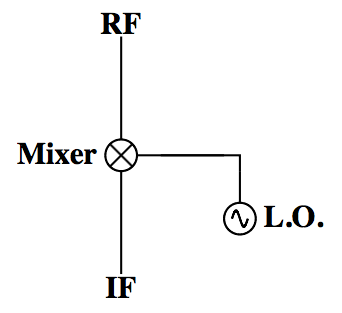
\includegraphics[height=2in]{dsbmixer.png}
\end{center}
%\vspace{-0.8in}
\caption{\footnotesize A DSB mixer. In the text, we sometimes refer to
  the RF input as the `signal'. \label{dsb}}
\end{figure}

In our lab, we have Mini-Circuits ZAD-1 and ZFM-15 mixers. 
They have three BNC connectors
labeled R, L, and X or I, corresponding to
the RF, LO, and IF, respectively.
Both the ZAD-1 and the ZFM-15 are
balanced mixers, so the R and L ports are identical but
{\it will not couple to DC or very low frequencies}.  To find out
the frequency ranges these mixers support on each input, 
look up the datasheet online. 

%In contrast,
%the ``I'' port is coupled differently and will handle voltages all the
%way down to, and including, DC.  The mixing process functions no matter
%which two ports are used as inputs.  For example, if you are using a
%mixer to modulate a high frequency (say, a few MHz) with a low frequency
%(say, a few kHz), you should use the ``I'' port for the low frequency
%and either of the other two for the high frequency; take the output from
%the third port.  

Use a mixer to build a DSB.
Assign a signal generator to
be your LO with frequency $\nu_{LO}$ and
another to be your RF signal with frequency $\nu_{RF} = \nu_{LO} \pm
\Delta \nu$.  Here, you choose the frequency difference $\Delta \nu$ and
you set the two signal generators 
for each of two cases:
$\nu_{RF} = \nu_{LO} + \Delta \nu$ and $\nu_{RF} = \nu_{LO} - \
\nu$.  Make $\Delta \nu$ small ($\sim5$\%) compared to $\nu_{LO}$.
For the input power level, a good choice is 0
dBm\footnote{What does this ``dBm'' mean? It is the power relative to 1
  milliwatt, expressed in decibels (dB).}
  for both synthesizers. The output consists of both the
sum and difference frequencies, so choose the ports appropriately.

Digitally sample the mixer output and identify the
sum and difference frequencies.
Consider
the Nyquist criterion and choose a sample rate. If you want enough samples per period to
produce a reasonable facsimile of the analog sine wave,
you may wish to sample at twice
Nyquist, or even faster.  Another parameter to consider is the number of points
sampled, which must be large enough to capture a few
periods of the slowest sine wave.

For the two cases $\nu_{RF} = \nu_{LO} \pm \Delta \nu$, plot the power
spectra versus frequency. Explain why the plots look the way they do. In
your explanation include the terms upper sideband and lower
sideband.

For one of the cases, plot the waveform.  Does it look like the
oscilloscope trace? Also, take the Fourier transform (not the power
spectrum) of the waveform and remove the sum frequency component by
zeroing both the real and imaginary portions (this is {\bf Fourier
filtering}).  Recreate the signal from the filtered transform by taking
the inverse transform and plot the filtered signal versus time.  Explain
what you see.

\subsection{Intermodulation Products in Real Mixers}

\noindent
An ideal mixer multiplies two input
signals, but real mixers are not ideal. Inside,
nonlinear diodes are used to perform an approximate multiplication, but
deviations from ideal behavior 
produce harmonics of the input signals and harmonics of the sum, and harmonics
of harmonics.
These undesired products are called
{\bf intermodulation products}.
When a well-designed
mixer is operated with the proper input signal levels, the intermods
have much less power than the main product, but they can nevertheless
ruin sensitive measurements.

Examine one of the power spectra obtained above using a logarithmic vertical
axis.
Do you see the forest of lines?
See if you can identify how some of the
stronger ones originate as harmonics of the main lines.

\subsection{ The Single-Sideband Mixer (SSB Mixer)}
\label{sectssb}

\noindent
A single sideband (SSB) mixer (Figure \ref{ssb}) is a
little more complicated than the DSB mixer. It consists of two identical
DSB mixers fed by an LO that is $90^\circ$ phase shifted in the right-hand mixer.
Hence, we can regard the left-hand output as being mixed with a cosine while
the right-hand side extracts the sine component.
together, they produce the real and imaginary components of a complex function
that can now produce power spectra that contain different information
at postive and negative frequencies.
Engineers call this IQ sampling.

\begin{figure}[h!]
\begin{center}
%\vspace{-0.7in}
  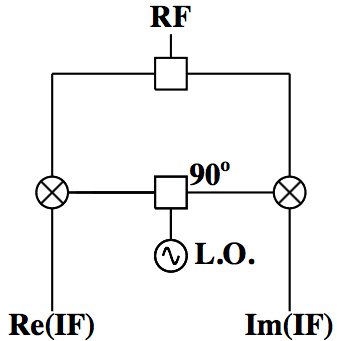
\includegraphics[height=2in]{ssbmixer.png}
\end{center}
%\vspace{-0.8in}
\caption{\footnotesize An SSB mixer. The important part is the
  $90^\circ$ phase delay in the right-hand LO, which is normally
  produced with a quadrature splitter, but we can make it
  with a $\lambda/4$ piece of cable. \label{ssb}}
\end{figure}

From the block diagram in Figure \ref{ssb}, construct an SSB mixer that
achieves the phase delay with a cable\footnote{In vaccuum, light travels
1 foot per nanosecond---the only legitimate use of
imperial units in astronomy. In a cable, light travels about
70\% slower than in vaccuum. You should be able to use this information
to get a ballpark estimate of a cable suits your
needs for a chosen frequency.}. We will use
it to experiment with no phase delay (a short cable) and a $90^\circ$
phase delay (a long cable).  For experimentation with this two-output
mixer, use two frequency synthesizers, as before.

\subsubsection{Reverting to a DSB Mixer} \label{dsbmixer}

\noindent
First see what happens when the phase delay cable is short (ideally
zero), so that the two halves of the SSB are essentially identical.
Pick a value for $\pm\Delta\nu$ and take time
series data for the two corresponding values of $\nu_{RF}$ (i.e., the
upper and lower sidebands). Calculate the power spectra. When taking the
Fourier transform, be sure to make assign the inputs to the real and imaginary
parts of a complex {\tt numpy} array.
Looking at the power spectra alone, can you distinguish between positive and negative $\Delta
\nu$?

\subsubsection{The SSB Mixer}

\noindent
Now see what happens when the phase delay cable introduces a 
phase delay of $90^\circ$ in the LO going to the right mixer.
Repeating the steps in \S \ref{dsbmixer},
can you distinguish between positive and negative
$\Delta\nu$ in the power spectra now?

If you have the time and inclination, verify the phase difference
between the two mixer outputs.
Why does it behave this way?  







\section {On Mixers and the Heterodyne
  Process (At Home, Week 2)} \label{hetereo}

%
\subsection{The Heterodyne Process}
%
\noindent
Mixers allow us to shift the frequency of the
whole input spectrum by a uniform amount.  They do this by multiplying
the input signal by a sine-wave {\bf local oscillator} (LO) with frequency
$\nu_{LO}$ (though we will often use
angular frequency, $\omega_{LO}$, for cleaner notation).

This is an important tool for RF signal chains (astronomical and otherwise)
because {\it antennas} must be tuned to the frequency of the incoming radiation they
target, but our filters, amplifiers, and samplers often must work at far lower
frequencies.

AM (amplitude-modulated) radio stations, for example, broadcast signals in the 1-MHz
range (for frequency-modulated FM stations, it is 100 MHz), but the information content
is music at audio (kHz) frequencies.
A mixer is used to shift the frequencies of
the AM station down to the audio region, where they are filtered off, amplified, and
sent to a speaker that converts the voltage fluctuations into pressure-wave fluctuations
that your ear is sensitive to.  When you tune in to a station, you are simply changing
the LO frequency; the rest of the signal chain can stay the same.

Such receivers are called {\bf heterodyne} receivers, and they are used 
in consumer radios, television (even modern digital ones), and cellphones, as well
as in more noble pursuits, like radio astronomy.
%
\subsection{Single Sideband (SSB) Mixer Theory}

\noindent
Even though we construct the SSB Mixer after the DSB in the lab, the theory of it
is easier to understand, provided we use
complex numbers and {\bf negative frequencies}.
Negative frequencies might seem weird. How can something oscillate
a negative number of times per second?

To understand, let us use
Euler's formula to write a complex sinusoid as
\begin{equation}
Ae^{iwt} = A\cos(\omega t) + i\cdot A\sin(\omega t).
\end{equation}
In some ways, this complex sinusoid is the ``true" sine wave.  The real-valued
versions are built out of pairs of complex sine waves:
\begin{align}
\cos(\omega t) &= \frac12(e^{i\omega t} + e^{-i\omega t}) \\
\sin(\omega t) &= \frac1{2i}(e^{i\omega t} - e^{-i\omega t})
\end{align}

Now, once we have defined a complex sine wave (which henceforth will just be
called a ``sine wave"), we can switch $-\omega$
for $\omega$,
\begin{equation}
Ae^{i(-w)t} = A\cos(\omega t) - i\cdot A\sin(\omega t),
\end{equation}
which is to say that the negation of a frequency swaps the sign of the imaginary 
component.  So rather than thinking of a negative frequency as ``negative Hertz",
let us instead think of it as a phase relationship between the sine and cosine components.

Now let's take an idealized SSB mixer that has a LO that
is a complex sinusoid $e^{-i\wLO t}$ of unity amplitude with a negative frequency.  
This LO is mixed (multiplied) by an input signal. As an example, let's take an input signal
that is the sum of two real-valued sine waves,
\begin{equation}
E(t)=A\sin (\wLO-\Delta\omega)t + B \sin (\wLO+\Delta\omega)t.
\end{equation}
We can then use Euler's formula to express the product output by the mixer as
\begin{align}
E(t)\cdot e^{-i\wLO t} &= A\sin (\wLO-\Delta\omega)t\cdot e^{-i\wLO t} + B \sin (\wLO+\Delta\omega)t \cdot e^{-i\wLO t}\\
&= \frac{A}{2i}\left[e^{i(\wLO-\Delta\omega)t}-e^{-i(\wLO-\Delta\omega)t}\right]e^{-i\wLO t} +
  \frac{B}{2i}\left[e^{i(\wLO+\Delta\omega)t}-e^{-i(\wLO+\Delta\omega)t}\right]e^{-i\wLO t}\\
&= \frac{A}{2i}\left[e^{-i\Delta\omega t}-e^{-i(2\wLO-\Delta\omega)t}\right] +
  \frac{B}{2i}\left[e^{i\Delta\omega t}-e^{-i(2\wLO+\Delta\omega)t}\right].
\end{align}
After mixing, each component sine wave in $E(t)$ has a beat-frequency term
$e^{\pm i \Delta\omega t}$, as well as a component at much higher frequency ($2\wLO$).
These higher-frequency components are typically filtered off using a low-pass filter (LPF), leaving just the
beat-frequency terms
\begin{equation}
{\rm LPF}\left[E(t)\cdot e^{-i\wLO t}\right] =
  \frac{A}{2i}e^{-i\Delta\omega t} + \frac{B}{2i} e^{i\Delta\omega t}.
\end{equation}
These terms retain the amplitude and frequency offset of their original signal, but have been shifted 
to lower frequencies where they can be easily sampled and processed%
\footnote{For a radio station, the signal is
speech or music which spans a range of $\Delta\omega$. In astronomy,
(e.g.\ the 21-cm line), the signal is a Doppler broadened line, which
again has a broad range of $\Delta\omega$.  In both cases, a mixer with a well-chosen
LO frequency can be used to mix the signal down to lower frequencies where it can
be sent to a speaker (if you are listening to the radio, or if you are Jodie Foster's
character {\it Ellie} in {\it Contact}.}.

Furthermore, so long as we retain both the real and imaginary components (which,
in reality, are just the components of the original signal that were multiplied by 
the cosine and sine components of the LO, respectively), we can distinguish 
between the $A$ and $B$ signal components by whether they appear at positive or negative
frequencies.  This ability to distinguish between positive and negative {\bf sidebands}
is why we call this a single-sideband mixer: we can look at each sideband separately.
If we didn't have both the cosine and sine components, we would not be able to distinguish
positive and negative frequencies. Signals $A$ and $B$ would then sit on top
of each other, and we would have no choice but to look at both sidebands simultaneously.

Figure\ \ref{ssb} shows a block diagram of the SSB mixer.  The RF input
and the LO are each split by a power splitter so that we have two
identical mixers, one on the left and one on the right, whose outputs
are labelled {\bf Re(IF)} and {\bf Im(IF)}, respectively. The one on
the left is identical to the DSB mixer in figure \ref{dsb}. The one on
the right differs in only one way, which is crucial: its LO is delayed
by $90^\circ$ relative to that on the left. With this, the {\bf Im(IF)}
output lags the {\bf Re(IF)}, becoming a sine wave to the {\bf Re(IF)}'s 
cosine.

%\begin{figure}[h]
%%        \begin{center}
%%\hspace{-0.5in}
%%        \leavevmode
%        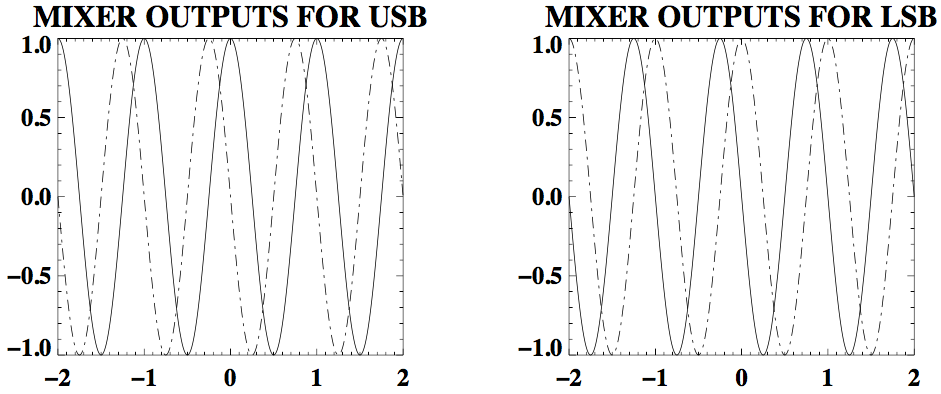
\includegraphics[width=6.5in]{ssbm.png}
%%        \end{center}
%\caption{Outputs of the first mixers for the two sideband cases. Dashed
%  curve shows the left-hand mixer, solid is the right-hand
%  mixer. Left panel shows $\Delta \omega > 0$ (upper
%  sideband---USB); right panel shows $\Delta \omega < 0$ (lower
%  sideband---LSB).
%\label{mixerout}}
%\end{figure}


\subsection {Double Sideband (DSB) Mixer Theory}
%
\noindent
We now turn to the theory of the DSB mixer, which
is very straightforward to build (the LO is just a real-valued sine wave, as is the RF, so we only
require one mixing circuit),
but is more complicated to understand.

Let us repeat the SSB derivation, but instead of
using $e^{-i\wLO t}$ as our LO, we will use $\sin \wLO t$.
If we take our signal to be $E(t)=A\sin(\wLO+\Delta\omega)t$.  In this case,
the output of our mixer becomes
\begin{align}
E(t)\cdot \sin\wLO t &= A\sin (\wLO +\Delta\omega)t\cdot \sin (\wLO t)\\
&= \frac{A}{2i}\left[e^{i(\wLO +\Delta\omega)t}-e^{-i(\wLO +\Delta\omega)t}\right]\cdot
  \frac{1}{2i}\left[e^{i\wLO t}-e^{-i\wLO t}\right] \\
&= \frac{A}{2}\left[e^{i\Delta\omega t}+e^{-i\Delta\wLO t} -
  e^{i(2\wLO +\Delta\omega) t}-e^{-i(2\wLO +\Delta\omega)t}\right]\\
&= A\left[\cos\Delta\omega t - \cos(2\wLO +\Delta)t\right].
\end{align}
As in the SSB, the mixer output has two components: a beat frequency (our
desired output) and a component near $2\wLO $ (which we remove using a LPF).

The unfortunate part about the DSB mixer becomes obvious if we consider the
case we used for the SSB mixer, where $E(t)=A\sin(\wLO +\Delta\omega)t + B\sin(\wLO -\Delta\omega)t$.
Repeating our algebra above, we find that
\begin{equation}
E(t)\cdot \sin\wLO t = 
A\left[\cos\Delta\omega t - \cos(2\wLO +\Delta)t\right] +
B\left[\cos(-\Delta\omega) t - \cos(2\wLO -\Delta)t\right].
\end{equation}
But $\cos(-\Delta\omega)t=\cos\Delta\omega t$, so after filtering off the high-frequency components,
we end up with
\begin{equation}
{\rm LPF}\left[E(t)\cdot \sin\wLO t\right] = (A+B)\cos\Delta\omega t,
\end{equation}
which has signals that were at two different frequencies 
($\wLO +\Delta\omega$ and $\wLO -\Delta\omega$)
stacked on top of each other.

The DSB mixer, though simpler to build, cannot distinguish between positive and negative deviations around
the LO frequency.  It stacks them right on top of each other, so that any frequency you look at in the output
can be the sum of two different signals.  This is what lends it the name ``double sideband".


\begin{figure}[p!]
%\begin{center}
%\hspace{-0.7in}
  
\includegraphics[width=6.5in]{sideband.png}
%\end{center}
%\hspace{-0.5in}
\caption{Upper (USB) and lower (LSB) sidebands in DSB and SSB mixers for a set of
test tones on top of broad level noise spectra. Panel 1 illustrates
  the RF
spectrum; panels 2 and 3 show the USB and LSB individually when
they undergo the DSB mixing process; panel 4 shows how they both add
together; panel 5 shows how the SSB mixer keeps them
separate. \label{sideband}}
\end{figure}
%
%Three things are important here:
%\begin{enumerate}
%
%\item The two sidebands---the two different input
%frequencies ($[\omega_{s-}= \wLO  - \Delta \omega]$ and $[\omega_{s+}=
%\wLO  + \Delta \omega]$)--- produce the same
%symmetric-around-zero pair of IF output frequencies $\pm |\Delta
%\omega|$. The DSB mixer
%cannot distinguish between the two input frequencies.
%
%\item Consider how $|\Delta \omega|$ depends on $\wLO $: for
%          the upper sideband, ${d |\Delta \omega| \over d\wLO } = -1$,
%          while for the lower $d {|\Delta \omega| \over d\wLO } =
%          +1$. We hope that the upper three panels of Figure
%          \ref{sideband} elucidate the situation.
%
%\item A value of $E_s$ for one sideband produces a certain mixer
%output power; the same value of $E_s$ for the other sideband
%produces the same power. With regard to power, the sidebands are {\it
%indistinguishable}.
%
%\end{enumerate}
%
%\noindent
Figure \ref{sideband} illustrates the result. The top panel shows the
original RF spectrum, which consists of signals above the LO (the upper
sideband; USB
signal) and below (the lower sideband; LSB). Suppose you use a filter to
eliminate the LSB, leaving only the USB. The second panel
shows the IF spectrum after DSB mixing: the USB appears at both negative
and positive frequencies and the spectrum is symmetric, meaning that the
negative frequencies give exactly the same result as the positive ones.

Now use a filter to eliminate the USB, leaving only the LSB;
the third panel shows the resulting IF spectrum.

Without any filters, then both the LSB and the USB
would appear in the IF spectrum, as in the fourth panel. 
With a DSB mixer, you can't distinguish between LSB and
USB. They are inextricably
mixed into a sum in the power spectrum.
However, the bottom panel shows that SSB 
mixing retains the sideband separation.

\section{Writing the Lab Report (Week 3)} \label{report}

\noindent
Please review the resources linked on AstroBaki and the guidelines
offered in class for generating your report. Remember that your write-up
is the basis for the majority of your grade in this class; make sure to
include high-quality plots and description, providing adequate background
and discussion such that one of your peers who has not taken this class would
be able to understand your findings and conclusions. Take the opportunity to
show off what you have learned so far!

Your report should directly address the goals listed in \S\ref{goals}, but
please ensure that you do so in a narrative that is directed toward the goal
of conveying high-level results.  It would be a mistake to make this report a
laundry-list of the things you did during the last couple of weeks. Not every
plot you made needs to be in this report, nor should every wrong turn be documented.
A scientific publication documents process, but only insofar as is necessary
to generate the results presented.

Finally, heed the warning that write-up takes longer than you think it will. Get
started early and allow yourself plenty of time.

%\subsection{Handouts}
%
%\begin{enumerate}
%\item What should your lab report look like? {\tt
%  labreport\_comments.pdf} {\it ``SUGGESTIONS FOR LAB REPORTS''}
%
%\item You must use \LaTeX for your lab report! {\tt sample.pdf} ``\LaTeX
%  Is Your Friend OR ENEMY?'' Answer to this question is a
%  resounding YES for `Friend'---if you have followed his handout. Use
%  \LaTeX for preparing your lab report!
%
%\item Now's the time for another look at efficient use of your text
%  editor, because if you learn the keystroke commands you'll be much
%  quicker and save lots of time further down the road.
%
%\item You'll need to show plots into your lab report. To do this you
%  make PDF files of your plots. %See {\tt bpidl.pdf} {\it ``BPPython---BASIC PLOTTING IN
%  %Python: PLOTS, MULTIPLE PLOTS, COLORS, MAKING POSTSCRIPT FILES''} Section 6.0.1.
%
%\end{enumerate}
\end{document}
